\chapter{Introducción}
\label{cap:introduccion}
\setcounter{page}{1}

En la última decada, la evolución tecnológica ha provocado una transformación radical en nuestra forma de vivir, trabajar y relacionarnos desempeñando la tecnología un papel fundamental en el avance de la sociedad e impulsando una serie de innovaciones que se extienden desde la invención de la rueda hasta la era digital contemporánea. 
\bigskip

Entre las diversas ramas de la tecnología, la robótica se destaca como una de las más prometedoras. Apareciendo como disciplina durante la década de los años 60 teniendo un crecimiento exponencial en las últimas décadas. Dos figuras clave en el desarrollo de la robótica fueron Jorge Devalo (1921-2011) y 
José Engarberare (1925-2015) considerados como padres de la robótica, quienes crearon el brazo robótico llamado Unimate \footnote{\textbf{Unimate}: \url{https://www.invent.org/blog/inventors/George-Devol-Industrial-Robot/}}
\newline 
\newline 
Definiendo asi la robótica como ciencia interdisciplinaria que combina diversas ramas de la ingeniería y ciencías de la computación, se encarga de la concepción, creación, funcionamiento, estructuración, fabricación y uso de los robots.
Así, un robot es un conjunto de sistemas informáticos que incluyen sensores, actuadores y ordenadores. Estos elementos permiten al robot ser programado para cumplir objetivos específicos y adaptarse a su entorno. Los sensores con los que está equipado el robot, como cámaras, LIDARs y sensores láser, le permiten recoger datos de su entorno. 
Los actuadores proporcionan al robot la capacidad de movimiento, mientras que los ordenadores ejecutan el software, es decir, los algoritmos diseñados 
para llevar a cabo tareas específicas como la navegación autonóma, la detencción de objetos o manipulación de objetos con sensores táctiles y de fuerza.
Estas tareas que pueden desempeñar pueden ser peligrosas, delicadas, sucias o monótonas (conocidas como las 4D's: dull,dirty, dangerous and dear) \footnote{\textbf{4Ds}:\url{https://www.forbes.com/sites/bernardmarr/2017/10/16/the-4-ds-of-robotization-dull-dirty-dangerous-and-dear/?sh=40bb6cec3e0d}}

\begin{figure} [H]
  \begin{center}
    \includegraphics[width=1.0\textwidth,height=0.45\textwidth]{figs/introducción/robot.png}
  \end{center}
  \caption{Definición de robot.}
  \label{fig:robot}
\end{figure}\

\bigskip
La robótica se puede dividir de diferentes formas, sin embargo la más común es entre robótica industrial y robótica de servicio:


\begin{itemize}
  \item \textbf{La robótica industrial}: Son los que se encargan del diseño, desarrollo de brazos robóticos y manipuladores. El entorno de trabajo de este tipo de robots es un entorno controlado, estando en 
  áreas protegidas por seguridad del operario. Sus tareas suelen ser pick and place, soldadura, ensamblado de piezas,pintado, manipulación. etc. 
  \item \textbf{La robótica de servicio}: Abarca entornos no controlados y más difíciles que los robots industriales, por ejemplo: conducción autónoma, vigilancia, seguridad, sanidad, educación y más tareas. 
\end{itemize}

\begin{figure} [h!]
  \begin{center}
    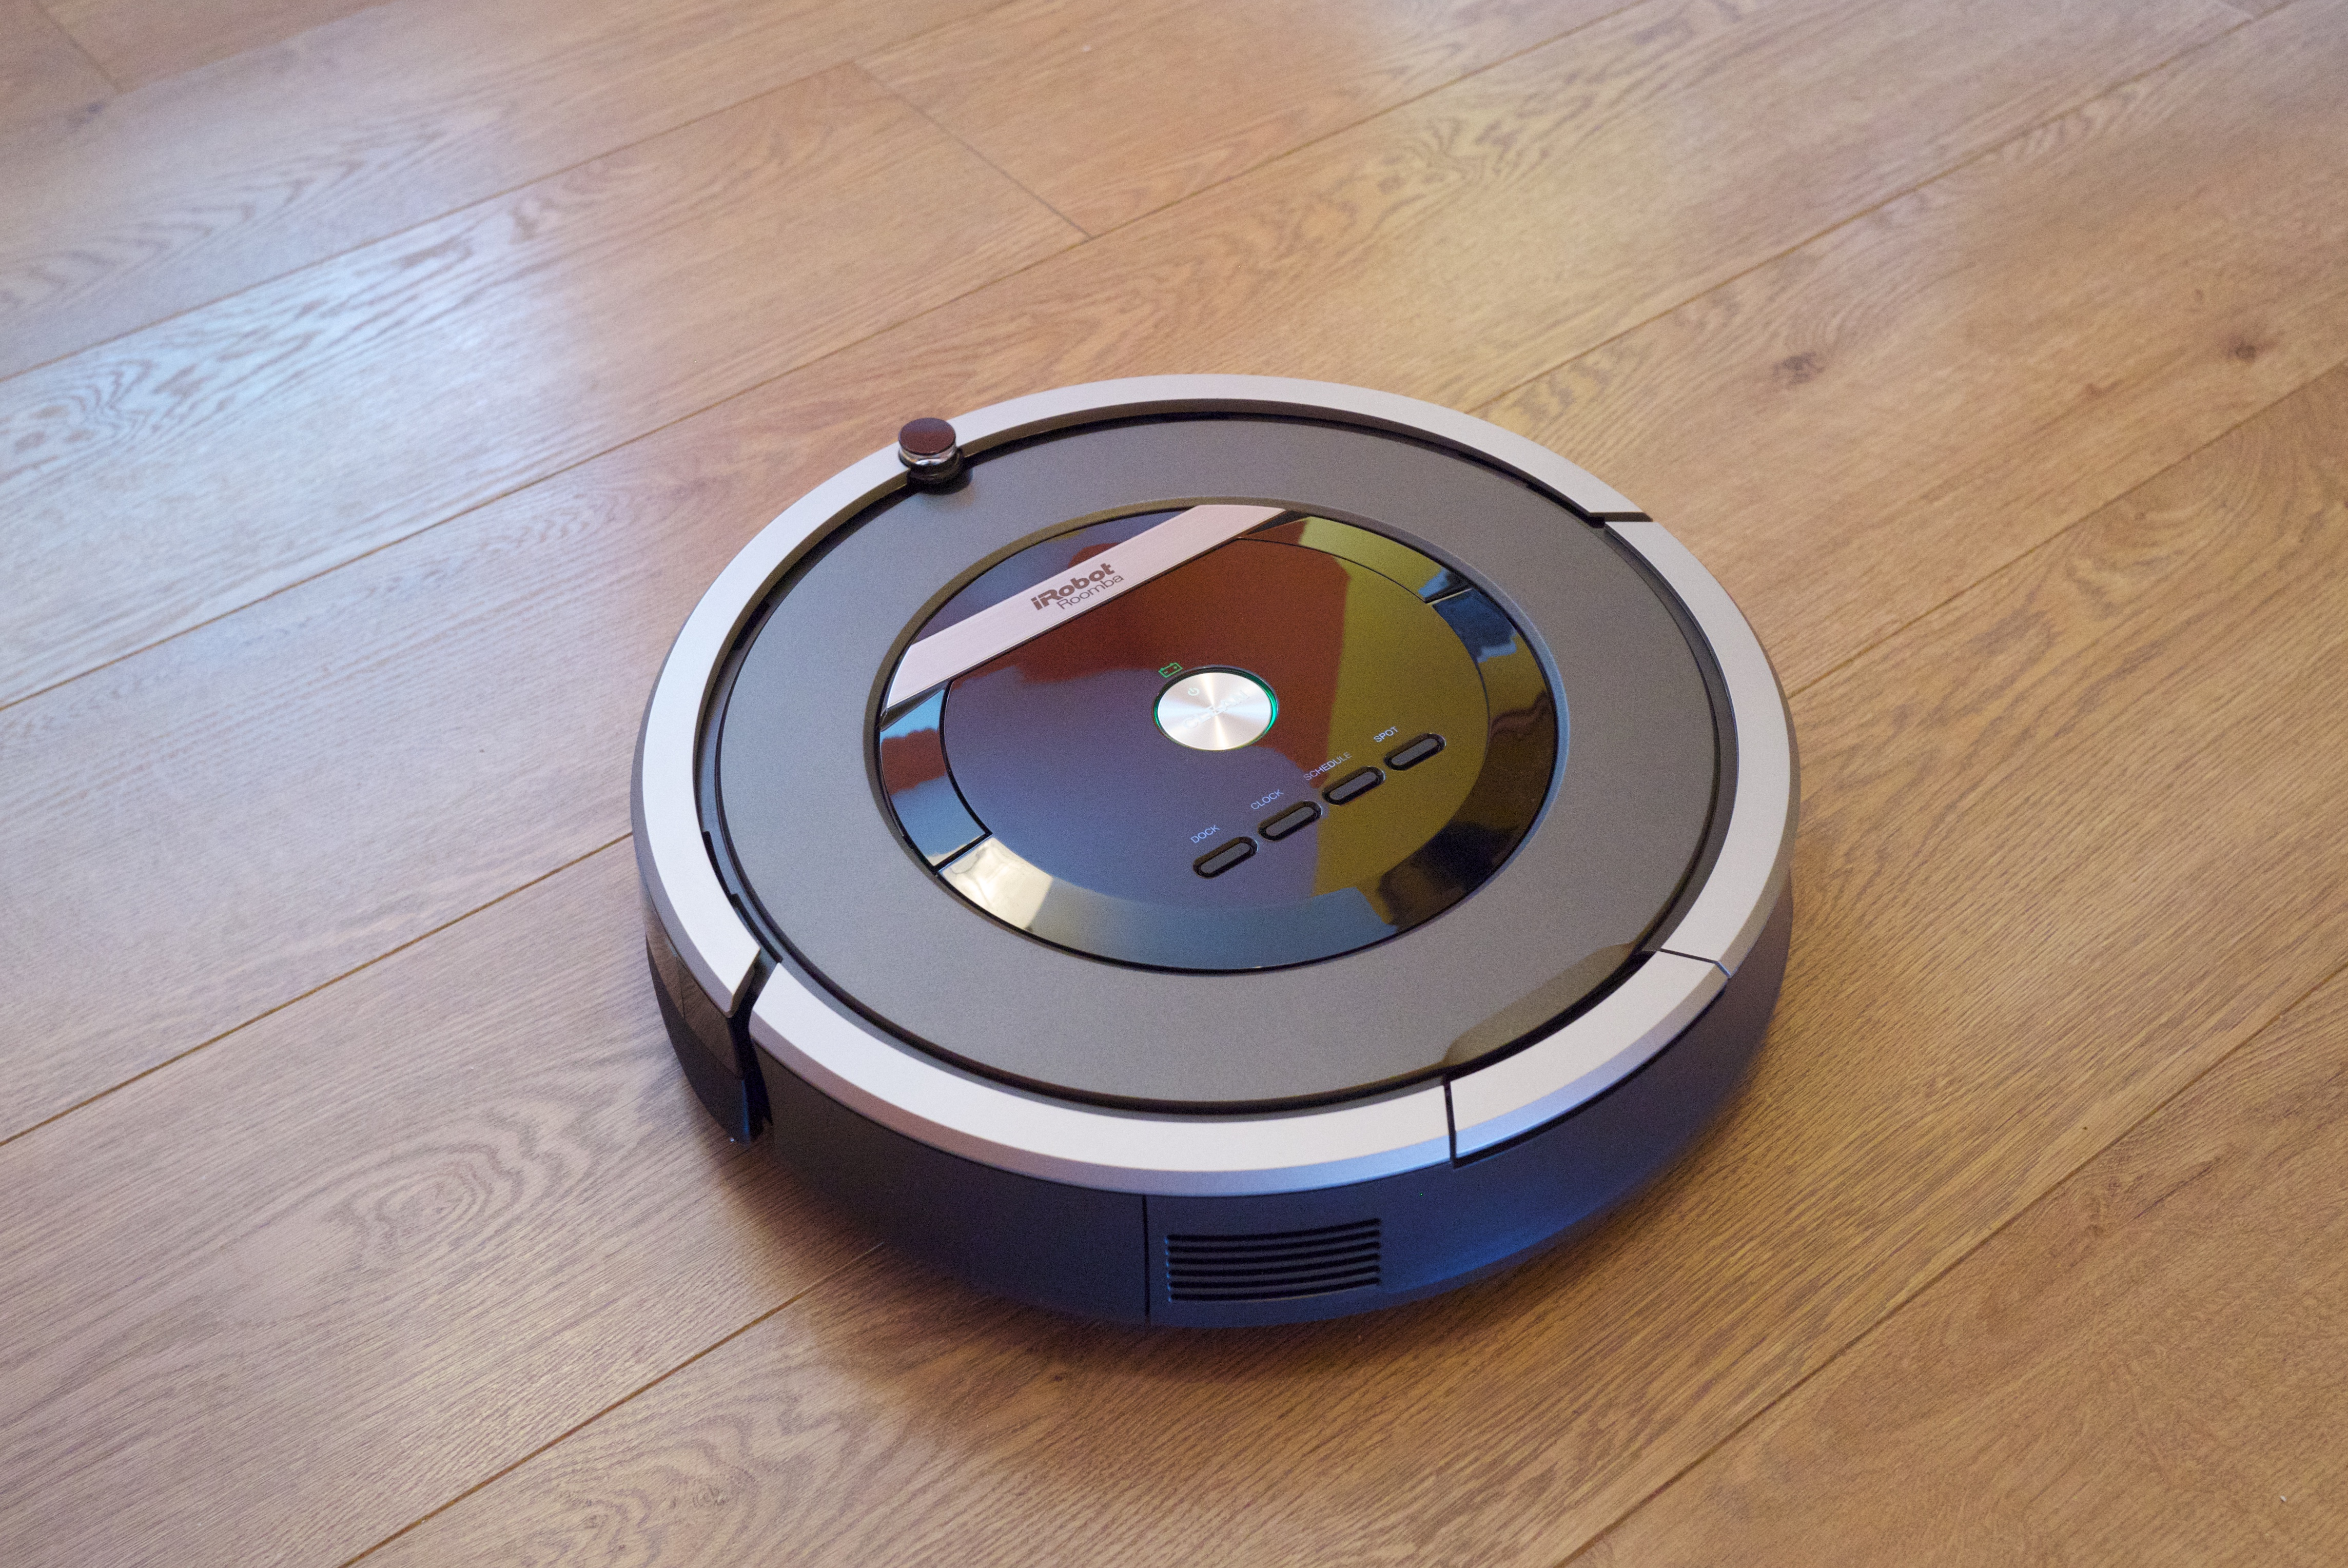
\includegraphics[width=0.3\textwidth,height=0.3\textwidth]{figs/introducción/roomba.jpg}
    \includegraphics[width=0.3\textwidth,height=0.3\textwidth]{figs/introducción/brazos_roboticos.jpg}
    \includegraphics[width=0.3\textwidth,height=0.3\textwidth]{figs/introducción/boston-dynamics-spot.jpg}
  \end{center}
  \caption{Robótica Industrial vs Robótica de servicio.}
  \label{fig:roomba}
\end{figure}\

En la categoría de robótica de servicio se encuentra los vehículos autónomos terrestres y aéreos. Ambos constan de sensores capaces de obtener información
de su entorno, dentro de los vehículos autónomos terrestres podemos tener los vehículos denominados AGV y AMR, principalemente su objetivo es mover
mercancia dentro de almaneces dentro de entornos industriales.
\newline
La gran diferencia entre los AGV y AMR\footnote{\textbf{AGV-VS-AMR}:\url{https://mobile-industrial-robots.com/es/blog/agv-vs-amr}} esta en la forma como realizan la navegación,los robots
que son AGV tienen caminos preestablecidos, esto quiere decir que tienen marcadores por el suelo facilitando su navegación pero esto conlleva a una desventajas
que seria la creación de todo el entorno de trabajo por ejemplo con líneas pintadas. \newline
En cambio los robots AMR son un tipo de vehículos autónomos mas sostificados 
que no necesitan marcadores en su entorno y equipado de más sensores que pueden realizar la evitación obstáculos utilizando ténicas de navegación variadas como SLAM\footnote{\textbf{SLAM}:\url{https://agvrobotics.es/navegacion-slam/}} .
\newline
\begin{figure} [h!]
  \begin{center}
    \includegraphics[width=0.4\textwidth,height=0.4\textwidth]{figs/introducción/AGV.jpg}
    \includegraphics[width=0.4\textwidth,height=0.4\textwidth]{figs/introducción/AMR.jpg}
  \end{center}
  \caption{AMR vs AGV.}
  \label{fig:AMR}
\end{figure}\

También dentro de los vehículos autónomos podemos tener coches autónomos dando servicio en restaurantes o repartiendo comida como el robot Nuro\footnote{\textbf{Nuro}: \url{https://www.nuro.ai/}}. 
Este robot esta equipado de sensores como una cámara estereo de 360 grados para poder visualizar a su alrededor, LIDAR para detectar obstáculos, permitiendo realizar
navegaciones autónomas con facilidady. Consta de un sistema de software denominado Nuro Driver\footnote{\textbf{Nuro Driver}: \url{https://medium.com/nuro/the-nuro-driver-1b17847fd261}} 
basado en IA y cálculos personalizados. Este software garantiza una condución segura y robusta para poder administrar las operaciones de entrega de manera efectiva. 

\begin{figure} [H]
  \begin{center}
    \includegraphics[width=0.4\textwidth,height=0.4\textwidth]{figs/introducción/Nuro.jpg}
  \end{center}
  \caption{Nuro}
  \label{fig:Nuro}
\end{figure}\

Junto a los vehículos autónomos terrestres existen los aéreos, como los drones. Estos vehículos se están
convirtiendo en una herramienta versátil por su autonomía, estabilidad y la capacidad de carga útil. Además, han demostrado ser útiles en situaciones donde
el acceso del ser humano puede llegar a ser peligroso y de difícil acceso, como la inspección de infraestructuras, el seguimiento de incendios o la vigilancia
de fronteras. Aparte de estas tareas, también los drones han abierto nuevas posibilidades en el mundo del entretenimiento con espectáculos que combinan
luces y coreografías aéreas. Estos eventos están ganando popularidad en eventos deportivos, conciertos o festivales. 

Los espectáculos de drones incluyen formaciones complejas y deben ser sincronizadas creando figuras en el cielo cautivando al público demostrando el potencial
artístico y técnico de esta tecnología. 

\begin{figure} [H]
  \begin{center}
    \includegraphics[width=0.7\textwidth,height=0.5\textwidth]{figs/introducción/drones-eventos.jpg}
  \end{center}
  \caption{Espectáculo de drones}
  \label{fig:Espectáculo de drones}
\end{figure}\


\newpage
\section{Robótica aérea}
\label{sec:robotica aerea} % etiqueta para luego referenciar esta sección

Dentro del campo de la robótica aérea tenemos los drones. Podemos definir un dron,como vehículo aéreo no tripulado (UAV), es un tipo de aeronave que puede operar sin la necesidad de un piloto humano a bordo. Estos dispositivos pueden ser manejados de manera remota por un operador humano o pueden seguir una ruta
preestablecida. \\

\subsection{Historia de los drones}
\label{sec:subseccion}
El origen de los drones se remonta a la Primera Guerra Mundial con el biplano Kettering Bug.
Este era un torpedo no tripulado de 240 kg (con una envergadura de 4,5 m, una longitud de
3,8 m y una altura de 2,3 m)\footnote{\textbf{KetteringBug}:\url{https://www.nationalmuseum.af.mil/Visit/Museum-Exhibits/Fact-Sheets/Display/Article/198095/kettering-aerial-torpedo-bug/}} era propulsado por un motor alternativo. Podía volar de
forma autónoma hasta un punto específico, donde soltaba sus alas y caía en “caída libre” \footnote{\textbf{KetteringBug}:\url{https://daytonunknown.com/2023/06/30/the-kettering-bug-the-worlds-first-drone/}}.\newline
Avanzando en la historia, en 1935 se desarrolló el DH.82 Queen Bee\footnote{\textbf{QueenBee}:\url{https://dronewars.net/2014/10/06/rise-of-the-reapers-a-brief-history-of-drones/}}. Este era un blanco aéreo sin piloto que era controlado por radio. De hecho, parece que el término “dron” se originó a partir del nombre, que se refiere a la abeja macho que realiza un vuelo en busca de la abeja reina y luego fallece. 

Durante la Segunda Guerra Mundial, quizás el más conocido fue el V-1 "Flying Bomb"\footnote{\textbf{V-1" FlyingBomb"}:\url{https://migflug.com/jetflights/the-v1-flying-bomb/}} , el primer misil
de crucero operativo del mundo, en donde su sistema de guía prestablecido incluía una brújula magnética que monitoreaba un autopiloto con giroscopios. También en este periodo, destacaremos el \textit{Proyect Aphrodite} \cite{Aphrodite}, fue un programa que tenía como objetivo convertir bombarderos en bombas voladoras no tripuladas que eran controladas por radio. Más adelante estos bombarderos no tripulados se utilizaron para volar a traves de nubes de hongo
después de las pruebas nucleares.

Destacando más UAVs, tenemos la familia Teledyne Ryan Firebee/Firefly \footnote{\textbf{TeledyneRyanFirebee/Firefly}:\url{https://www.designation-systems.net/dusrm/m-34.html}}, estos sistemas generalmente se lanzaban desde el aire y se recuperaban mediante una combinación de paracaidas y helicopteros. El Lockheed D-21 fue uno de los sistemas más impresionantes durante la Guerra Fría. Este UAV fue propulsado por estatorreactor con velocidades mayores que Mach 3 \footnote{\textbf{LockheedD-21}:\url{https://www.marchfield.org/aircraft/unmanned/d-21-drone-lockheed/}} . En la Edad Moderna, destacamos El Condor \cite{CondorUAV}, fue el primer UAS en utilizar navegación GPS y tecnología de aterrizaje automático y el Predactor \footnote{\textbf{Predactor}:\url{https://www.airforce-technology.com/projects/predator-uav/?cf-view}}. 
En la época dorada, gracias a los avances anteriores se pudo desarrollar sistemas militares esenciales que han demostrado su valor y el desarrollo de vehículos aéreos no tripulados pequeños (small UAV). Este ultimo ha despertado un gran interés significativo resaltando como puntos de entrega al mercado civil. 

\begin{figure}[H]
  \begin{center}
    \subfigure[Kettering Bug]{
     \includegraphics[width=0.3\textwidth,height=0.2\textwidth ]{figs/introducción/historia_drones/kettering-bug.jpg}
     \label{f:Kettering Bug}}
    \subfigure[Queen Bee]{
     \includegraphics[width=0.3\textwidth,height=0.2\textwidth ]{figs/introducción/historia_drones/queen-bee.jpg}
     \label{f:Queen Bee}}
    \subfigure[V-1]{
      \includegraphics[width=0.3\textwidth,height=0.2\textwidth ]{figs/introducción/historia_drones/V-1.jpg}
      \label{f:V-1 "Flying Bomb"}}
    \subfigure[Proyect Aphrodite]{
      \includegraphics[width=0.3\textwidth,height=0.2\textwidth ]{figs/introducción/historia_drones/proyect-aphorite.jpg}
      \label{f:Proyect Aphrodite"}}
    \subfigure[Teledyne Ryan Firebee/Firefly]{
      \includegraphics[width=0.3\textwidth,height=0.2\textwidth ]{figs/introducción/historia_drones/Firebee.jpg}
      \label{f:Teledyne Ryan Firebee/Firefly"}}
    \subfigure[Lockheed D-21]{
      \includegraphics[width=0.3\textwidth,height=0.2\textwidth ]{figs/introducción/historia_drones/The_Lockheed_D-21.jpg}
      \label{f:Lockheed D-21"}}
    \subfigure[El Condor]{
      \includegraphics[width=0.3\textwidth,height=0.2\textwidth ]{figs/introducción/historia_drones/Boeing-Condor-UAV-23.png}
      \label{f:El Condor"}}
    \subfigure[Small UAV]{
      \includegraphics[width=0.3\textwidth,height=0.2\textwidth ]{figs/introducción/historia_drones/small-UAV.jpg}
      \label{f:small-UAV"}}
    \subfigure[Dron]{
      \includegraphics[width=0.3\textwidth,height=0.2\textwidth ]{figs/introducción/historia_drones/dron.jpg}
      \label{f:dron"}}
  \caption{Historia de los drones}
  \label{f:Drones}
  \end{center}
 \end{figure}

\newpage
\subsection{Componentes de un UAS}
\label{sec:UAS}

Como hemos descrito anteriormente en la historia, podemos definir UAS como : 

\begin{enumerate}
  \item \textbf{UAV}: Vehículo aéreo no tripulado 
  \item \textbf{Ground Control Station (GCS)}: Se trata de una estación de control terrestre o marítimo que proporciona el control de la aeronave
  \item \textbf{Comunicaciones}: Consiste en la gestión de datos y conectividad entre el UAV y la GCS a través de links o canales de transmisión. Dentro de las comunicaciones podemos tener 2 tipos: 
  \begin{itemize}
    \item  \textbf{Line-of-Sifht (LOS)}: Requiere una linea directa de visión entre el transmisor y el receptor, es decir, sin obstáculos físicos 
    \item  \textbf{Beyond-Line-of-sight (BLOS)}: Permite tener una transmisión más allá de la linea de visión directa.En otras palabras, tanto el transmisor como el receptor no necesitan estar en la linea de vision directa. Entre ellos puede haber comunicación satelital. 

  \end{itemize}
\end{enumerate}

\begin{figure}[H]
  \begin{center}
    \includegraphics[width=0.8\textwidth,height=0.5\textwidth]{figs/introducción/UAS/UAS.png}
  \end{center}
  \caption{Ilustración de UAS}
  \label{fig:uas}

  
\end{figure}

\newpage
\subsection{Aplicaciones de drones dentro del mundo de la robótica}
\label{Aplicaciones de los drones}
Dependiendo de las tareas a realizar, los drones pueden variar en tamaño, peso y capacidad de
carga útil y también por su marco legislativo. Es importante destacar que la elección del dron
adecuado dependerá en gran medida de las necesidades específicas de la tarea en cuestión. \\

Por lo tanto, es esencial tener en cuenta estos factores al seleccionar un dron para un
propósito específico. Una de las grandes ventajas del uso de vehículos aéreos son que pueden
realizar tareas con mayor rapidez y eficacia que los humanos en determinadas situaciones por
ejemplo en lugares peligrosos o inaccesibles, como zonas catastróficas o terrenos escarpados,
lo que permite una mejor supervisión y recopilación de datos.\hfill
Aunque presentan desventajas como la seguridad, a medida que los drones se vuelven más
comunes en nuestro día a día, aumentan los riesgos asociados al mal uso, ya que pueden
provocar interferencias con el espacio aéreo, colisiones. Pueden verse afectados con
determinadas condiciones climatológicas, también en interiores (señales GPS), entre otros. \\

En relación con la robótica y los drones, hay múltiples ejemplos de aplicaciones, como por
ejemplo  “\textit{follow person}” \cite{PersonFollowing} el cual consiste en detectar y moverse al ritmo de la persona.
Otro tipo de aplicación podría ser la entrega de paquetes mediante el proyecto de Amazon PrimeAir \cite{AmazonPrimeAir}.
Además de estas aplicaciones, los drones también se utilizan en una variedad de campos como
la agricultura con el uso de la Inteligencia Artificial, detectando plagas, malas hierbas o
plantación. \\

En resumen, los drones son una tecnología emergente con un potencial significativo para
transformar una variedad de industrias. Sin embargo, también plantean desafíos únicos que
deben ser abordados a medida que se integran más plenamente en nuestra sociedad. Con el
desarrollo continuo de la tecnología de los drones y la evolución de las regulaciones, es
probable que veamos un aumento en la variedad de las aplicaciones de los
drones en el futuro.

\newpage
\section{Inteligencia Artificial}
\label{sec:IA}

La inteligencia artificial ha tenido un crecimiento considerable en estos últimos años, desde la
prueba de Turing propuesta por Alan Turing (1950) “Computing Machinery and Intelligence” \footnote{\textbf{Computing Machinery and Intelligence}: \url{https://www.cse.chalmers.se/~aikmitr/papers/Turing.pdf}},
que consistía en un experimento en el cual una persona entablaba una conversación y
tenía que averiguar al final del experimento si se trataba de una persona o una máquina,
gracias a este experimento impulsó el desarrollo de máquinas que pueden imitar el
comportamiento humano hasta llegar al punto de cuestionarnos de sí se trata de una máquina
o un humano, hasta en la actualidad con el desarrollo de la navegación autónoma de vehículos
a través del aprendizaje o chatbots como ChatGPT o Bing. \\

\begin{figure} [H]
  \begin{center}
    \includegraphics[width=0.5\textwidth,height=0.5\textwidth]{figs/introducción/IA/Test-Turing.jpg}
  \end{center}
  \caption{Ilustración del test de Turing}
  \label{fig:Turing}
\end{figure}

Dentro de la IA, tenemos las redes neuronales artificiales, que consisten en imitar el
comportamiento del cerebro humano a través de neuronas y las conexiones que puede haber
en ellas. Una de las grandes aplicaciones de las redes neuronales centrándonos en la robótica
puede ser el reconocimiento visual en los vehículos autónomos para reconocer las señales de
tráfico o fijándonos en drones, pueden desempeñar tareas a través con redes neuronales de
búsqueda y rescate, proporcionando una vista aérea en la cual puedan localizar personas
perdidas o en peligro. 

\begin{figure} [H]
  \begin{center}
    \includegraphics[width=0.7\textwidth,height=0.5\textwidth]{figs/introducción/IA/red-neuronal.jpeg}
  \end{center}
  \caption{Ilustración de una red neuronal }
  \label{fig:redneuronal}
\end{figure}

Existen múltiples formas de clasificar la Inteligencia Artificial, pero si nos centramos en el
Machine Learning, se pueden clasificar de la siguiente forma: 

\begin{enumerate}
  \item \textbf{Aprendizaje Supervisado}: Consiste en tener un conjunto de datos de entrada y su salida correspondiente y a través del algoritmo de aprendizaje pueda “aprender” la
  relación que hay entre la salida y el conjunto de entradas. Las aplicaciones de este tipo
  de aprendizaje se dividen en regresión y en clasificación. 
  \begin{itemize}
    \item \textbf{Regresión}: Un ejemplo de regresión, podemos tener la predicción del valor de la velocidad lineal y angular de un robot móvil a partir de los datos de los sensores de distancia (sónar) ubicados en el frontal del robot, de esta manera el robot podría predecir su propia trayectoria y navegar de una manera más eficiente
    \item \textbf{Clasificación}: un ejemplo de clasificación podemos tener la predicción
    del tipo de animal a partir de una imagen en color.
  \end{itemize}
  \item \textbf{Aprendizaje no Supervisado}: Consiste en únicamente tener un conjunto de datos de
  entrada y no tener datos de salida,con el fin de que el algoritmo de aprendizaje
  detecte patrones y estructuras de interés del conjunto de datos proporcionados.
  Podemos tener como aplicaciones en este tipo de aprendizaje el clustering
  (segmentación) y también se utiliza en menor medida como método para reducir la
  dimensionalidad de los datos. 
  Un ejemplo de clustering, podríamos tener un robot que obtenga de sus sensores
  datos de su entorno, por ejemplo, la temperatura, la humedad, la luz, etc. Con este
  tipo de algoritmo se podría agrupar todos estos datos en diferentes clústeres. Cada
  clúster representaría un “estado” del entorno lo cual de esta manera el robot podría
  entender mejor su entorno y adaptar su comportamiento en consecuencia.
  \item \textbf{Aprendizaje por Refuerzo}: Este tipo de aprendizaje consiste tener un algoritmo que
  aprenda a desarrollar la tarea encomendada a base de un esquema de recompensas y
  penalizaciones ante las decisiones que toma el algoritmo en cada una de las
  iteraciones. \newline

  Como ejemplo de aplicación podemos tener QT-Opt \cite{QTOpt}, desarrollado por
  Google en 2018, consiste en un brazo manipulador robótico el cual el robot aprende a
  manipular el objeto y aprender su propia estrategia de agarre.

  \begin{figure} [H]
    \begin{center}
      \includegraphics[width=0.7\textwidth,height=0.5\textwidth]{figs/introducción/IA/machine-learning.png}
    \end{center}
    \caption{Clasificación de Machine Learning }
    \label{fig:machinelearning}
  \end{figure}

  



\end{enumerate}



